\section{Cobertura: volatilidad implicita vs real}
Esta sección se centra en el caso en el que la volatilidad implícita es diferencte a la volatilidad que se ha calculado a partir de los datos históricos.
Si se compra un ATM strandle, el beneficio esperado es aproximadamente de
\[
\sqrt{\frac{2(T-t)}{\pi}}\, (\sigma - \tilde{\sigma})\, S.
\]
con una desviación típica de
\[
\sqrt{1 - \frac{2}{\pi}}\, \sigma S \sqrt{T-t}.
\]
donde $\sigma$ es la volatilidad real y $\tilde{\sigma}$ es la volatilidad implícita. La desviación depende de la volatilidad y tiene la misma magnitud que la media, por lo que el riesgo es muy alto, por lo que se debe seguir alguna estrategia para minimizar riesgos.

\begin{notation}
    Se define la $a$ superíndice para la volatilidad real y la $i$ como superíndice para la volatilidad implícita. Por ejemplo, $V^a$ es la delta usando la volatilidad real en la fórmula y $V^i$ es la delta usando la volatilidad implícita en la fórmula.
\end{notation}

Según sobre que volatilidad se decida hacer la cobertura, se obtiene distintos resultados:
\begin{itemize}
    \item \textbf{Cobertura sobre la volatilida real}: Sea el modelo
    \[
        dS = \mu S dt + \sigma S dX.
    \]
    se construye una cartera comprando la opción por $V^i$ y cubriendo con $\Delta^a$ del subyacente, lo que da lugar a un efectivo de $-V^i + \Delta^a S$. Es decir las cartera es:
    \begin{table}[H]
        \centering
        \begin{tabular}{l|c}
            \textbf{Componente} & \textbf{Valor} \\
            \hline
            Opción & $V^i$ \\
            Acción & $-\Delta^a S$ \\
            Efectivo & $-V^i + \Delta^a S$ \\
        \end{tabular}
    \end{table}
    \[
        \Pi = V^i-\Delta^a S-V^i + \Delta^a S
    \]
    Se supone además unos dividendos continuos de $D$ y una tasa de interés $r$. Entonces, la variación de la cartera es
    \[
        d\Pi = dV^i - \Delta^a dS - r(V^i - \Delta^a S)dt - \Delta^a D S dt
    \]
    Asumiendo que la opción está correctamente valorada en $V^a$, se tiene que
    \begin{align*}
        &dV^a - \Delta^a dS - r(V^a - \Delta^a S)dt - \Delta^a D S dt = 0 \Rightarrow \\
        \Rightarrow  &-\Delta^a dS - \Delta^a D S dt = -dV^a + r(V^a - \Delta^a S)dt
    \end{align*}
    por lo que sustituyendo en la variación de la cartera se obtiene
    \begin{align*}
        d\Pi &= dV^i - r(V^i - \Delta^a S)dt -dV^a - r(V^a - \Delta^a S)dt \\
        &= dV^i - dV^a - r(V^i - V^a)dt
    \end{align*}
    Se sabe que
    \begin{align*}
        &\frac{d}{dt} \left( e^{-rt}(V^i - V^a)\right) = -r e^{-rt}(V^i - V^a) + e^{-rt}\left(\frac{d}{dt}V^i - \frac{d}{dt}V^a\right) \Rightarrow \\
        \Rightarrow & d(e^{-rt}(V^i - V^a)) = e^{-rt}\left( -r(V^i - V^a)dt + dV^i - dV^a \right) \Rightarrow \\
        \Rightarrow & e^{rt}d(e^{-rt}(V^i - V^a)) = -r(V^i - V^a)dt + dV^i - dV^a \Rightarrow \\
    \end{align*}
    que sustituyendo en la variación de la cartera se obtiene
    \begin{align*}
        d\Pi &= dV^i - dV^a + e^{rt}d(e^{-rt}(V^i - V^a)) + dV^a - dV^i \\
        &= e^{rt}d(e^{-rt}(V^i - V^a))
    \end{align*}
    que actualizada actualizada a tiempo $t_0$ es
    \begin{align*}
        d\Pi &= e^{-r(t-t_0)}e^{rt}d(e^{-rt}(V^i - V^a)) \\
        &= e^{rt_0}d(e^{-rt}(V^i - V^a))
    \end{align*}
    La ganacia total desde $t_0$ hasta el vencimiento es
    \begin{align*}
        \int_{t_0}^T d\Pi &= \int_{t_0}^T e^{-rt_0}d(e^{rt}(V^i - V^a))\\
        &= e^{-rt_0}\left[ e^{rT}(V^i(T) - V^a(T)) - e^{rt_0}(V^i(t_0) - V^a(t_0))\right] = \\
        &= e^{-rt_0}\left[ - e^{rt_0}(V^i(t_0) - V^a(t_0))\right]
    \end{align*}
    Por lo tanto, el beneficio total garantizado al vencimiento es
    \[
        \boxed{V^a(t_0) - V^i(t_0) }
    \]
    Se debe de tener en cuenta que el beneficio final está garantizado, pero los beneficios en el camino son aleatorios.

    Se puede desmostrar que la variación de la cartera tambien se puede escribir como
    \[
        \frac{1}{2}(\sigma^2 - \tilde{\sigma}^2)S^2 \Gamma^i dt + (\Delta^i - \Delta^a)\left((\mu - r + D)S dt + \sigma S dX\right)
    \]
    
    \item \textbf{Cobertura sobre la volatilidad implícita}:Se usa igualmente el modelo
    \[
        dS = \mu S dt + \sigma S dX
    \]
    y se construye la cartera
    \[
        \Pi = V^i-\Delta^i S-V^i + \Delta^i S
    \]
    Sabiendo que hay un dividendos continuos, entonces su variación es
    \begin{align*}
        d\Pi &= dV^i - \Delta^i dS - r(V^i - \Delta^i S)dt - \Delta^i D S dt \\
        &= \Theta^i dt + \frac{1}{2} \sigma^2 S^2 \Gamma^i dt - r(V^i - \Delta^i S)dt - \Delta^i D S dt \\
        &= \frac{1}{2}(\sigma^2 - \tilde{\sigma}^2)S^2 \Gamma^i dt
    \end{align*}
    que actualizada a tiempo $t_0$ es
    \[ 
        d\Pi = e^{r(t-t_0)}\frac{1}{2}(\sigma^2 - \tilde{\sigma}^2)S^2 \Gamma^i dt
    \]
    \begin{figure}[H]
        \centering
        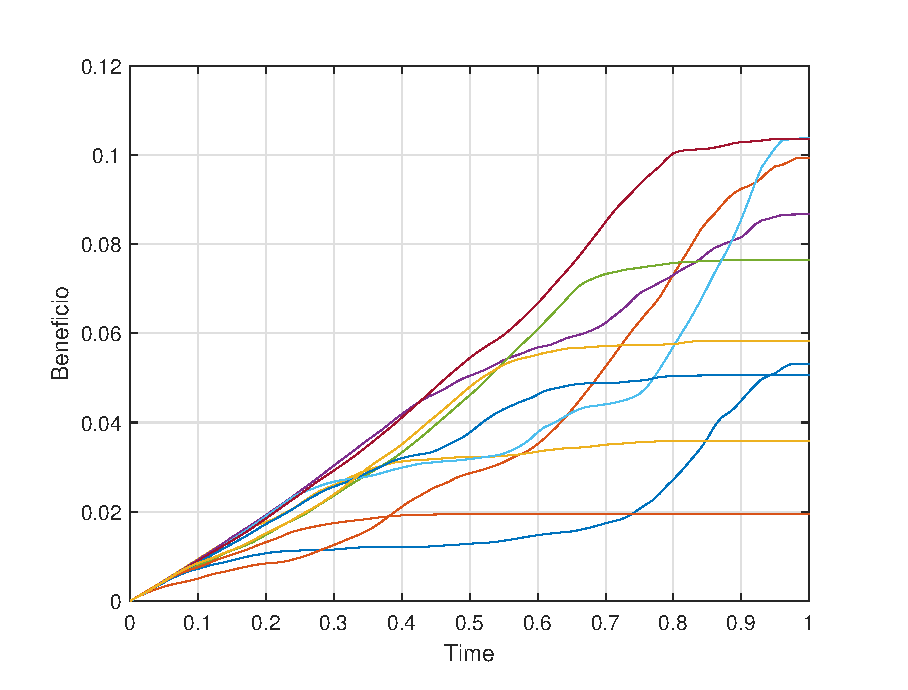
\includegraphics[width=0.65\linewidth]{Imagenes/10_Cobertura/Cobertura_Volat_Imp.eps}
        \caption{Beneficios de cobertura sobre la volatilidad implícita}
    \end{figure}
    por lo que en tiempo final hay un beneficio debe ser
    \[
        \boxed{\int_{t_0}^T d\Pi = \frac{1}{2}(\sigma^2 - \tilde{\sigma}^2) \int_{t_0}^T e^{r(t-t_0)}S^2 \Gamma^i dt}
    \]
    que es siempre positivo si la volatilidad real es mayor que la implícita. Se puede calcular la media y varianza de este beneficio. Para mas información, ver el apéndice~\ref{ApexCobVolImp}.

    Por lo tanto, el beneficio solo depende de gamma, por lo que las opciones put call tienen el mismo beneficio esperado. Si se construyen carteras con opciones con distintos strikes, se obtiene un beneficio de
    \[
        \frac{1}{2}\sum_k(\sigma^2 - \tilde{\sigma_k}^2) \int_{t_0}^{T_k} e^{r(t-t_0)}S^2 \Gamma^i_k dt
    \]
    cuya media y varianza se pueden calcular.
    \item \textbf{Cobertura cuando la volatilidad implícita es aleatoria}: Sean los modelos
    \begin{align*}
        dS &= \mu S dt + \sigma S dX_1 \\
        d\tilde{\sigma} &= a dt + b dX_2
    \end{align*}
    y la correlación $\rho$ entre $dX_1$ y $dX_2$.
    \begin{itemize}
        \item \textbf{Cobertura sobre la volatilidad real}: Usando los mismo argumentos que antes, se llega a que el beneficio final está asegurado. Por otro lado, la variación de la cartera está
        \begin{align*}
            d\Pi =& \frac{1}{2}(\sigma^2 - \tilde{\sigma}^2)S^2 \Gamma^i\, dt + (\Delta^i - \Delta^a)\left( (\mu - r + D)S\, dt + \sigma S\, dX_1 \right) + \\
            &+\frac{\partial V^i}{\partial \tilde{\sigma}}\, d\tilde{\sigma} + \frac{1}{2} b^2 \frac{\partial^2 V^i}{\partial \tilde{\sigma}^2}\, dt + \rho \sigma b S \frac{\partial^2 V^i}{\partial S \partial \tilde{\sigma}}\, dt.
        \end{align*}
        \item \textbf{Cobertura sobre la volatilidad implícita}: Usando los mismos argumentos que antes se llega a que la variación de la cartera está
        \begin{align*}
        d\Pi =&dV^i - \Delta dS - r(V^i - \Delta S)dt - \Delta D S dt\\
        =& \Theta^i dt + \Delta^i dS + \frac{1}{2} \sigma^2 S^2 \Gamma^i dt + \frac{\partial V^i}{\partial \tilde{\sigma}} d\tilde{\sigma} + \frac{1}{2} b^2 \frac{\partial^2 V^i}{\partial \tilde{\sigma}^2} dt \\
        &+ \rho \sigma b S \frac{\partial^2 V^i}{\partial S \partial \tilde{\sigma}} dt - \Delta dS - r(V^i - \Delta S)dt - \Delta D S dt.
        \end{align*}
        se puede obtener su esperanza y varianza.
    \end{itemize}
\end{itemize}

\subsection{Comportamiento de la volatilidad implícita}
Existen varios ``modelos'' de cómo se comporta la volatilidad implícita:
\begin{itemize}
    \item \textbf{Sticky Strike}: es constante para cada opción (i.e.\ para cada strike y vencimiento). Es común en los mercados de renta variable. Si la volatilidad implícita difiere de la volatilidad real se pueden obtener beneficios como se ha explicado.
    \item \textbf{Sticky Delta}: depende de su moneyness ($\xi = S/E$). Es común en mercados como el FX, donde se cotizan precios y volatilidades para opciones con deltas específicas. Se modela como $\tilde{\sigma} = g(\xi, t)$ por lo que:
    \[
        d\tilde{\sigma} = \left( \frac{\partial g}{\partial t} + \mu \frac{S}{E} \frac{\partial g}{\partial \xi} + \frac{1}{2} \sigma^2 \frac{S^2}{E^2} \frac{\partial^2 g}{\partial \xi^2} \right) dt + \sigma \frac{S}{E} \frac{\partial g}{\partial \xi} dX_1,
    \]
    La variación de la volatilidad implícita está perfectamente correlacionada con el subyacente, permitiendo una cobertura perfecta en términos de mark-to-market.

    Hay una variantes donde la volatilidad implícita depende de la volatilidad ATM y de una función del moneyness, por ejemplo:
    \[
        \tilde{\sigma} = \sigma_{ATM} \, g\left( \frac{\log(S/E)}{\sqrt{T-t}} \right).
    \]
\end{itemize}





